
作为软件开发中的常用工具,CMake可以与各种IDE和源代码编辑器集成。在使用IDE或编辑器的同时,这样的集成对用户来说可能会更方便。本节中,将介绍CMake如何与一些流行的IDE和编辑器的集成。

若希望获得关于如何使用IDE或编辑器的指南,这一节将不会涉及这些内容。本节的主要重点是研究和学习CMake与这些工具的集成。本节假设读者已有使用将要交互的IDE/编辑器的经验。

先从Visual Studio开始吧!

\subsubsubsection{2.4.1\hspace{0.2cm}Visual Studio}

Visual Studio是支持CMake的后来者之一。与其他流行的IDE不同,Visual Studio直到2017年才原生支持CMake。那一年,微软决定采取行动,引入了对处理CMake项目的内置支持,并发布了Visual Studio 2017。从那时起,内置支持CMake就成为了Visual Studio IDE的一个可靠特性。

开始介绍前,请获取一份Visual Studio 2017或更高版本的副本,对于老版本的Visual Studio没有这个特性。我们的例子中,将使用Visual Studio 2022社区版。

\hspace*{\fill} \\ %插入空行
\noindent
\textbf{从头开始创建一个CMake项目}

Visual Studio项目创建特性是基于项目模板的。在VS2017及以上版本中,项目模板也包含一个CMake项目模板。我们将学习如何使用这个模板来创建新的CMake项目。

要用Visual Studio创建一个新的CMake项目,请单击欢迎页面上的create a new project按钮。或者,可以通过在主IDE窗口中单击File | New | Project来访问,或者使用Ctrl + Shift + N (New Project)快捷键。VS2022的欢迎界面是这样的:

\begin{center}
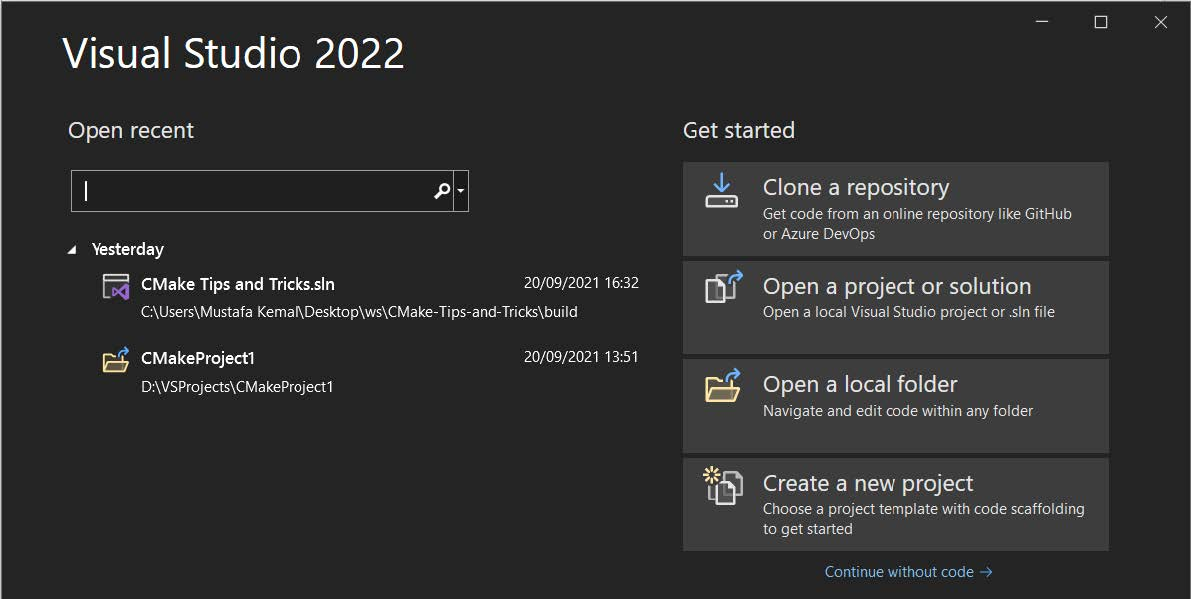
\includegraphics[width=0.8\textwidth]{content/1/chapter2/images/35.jpg}\\
图2.35 Visual Studio 2022欢迎界面
\end{center}

在“创建新项目”窗口上,双击项目模板列表中的CMake project。可以使用位于列表顶部的搜索栏来筛选项目模板:

\begin{center}
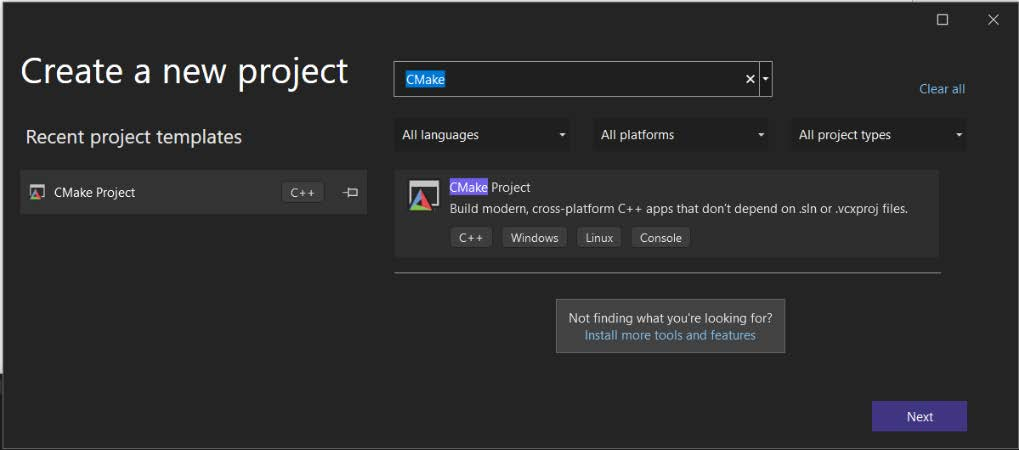
\includegraphics[width=0.8\textwidth]{content/1/chapter2/images/36.jpg}\\
图2.36 - Visual Studio 2022创建新项目界面
\end{center}

单击Next之后,将出现项目配置窗口。可以给CMake项目起一个名字,并选择将新项目放在哪里。在我们的示例中,将使用默认项目名称CMakeProject1。

\begin{center}
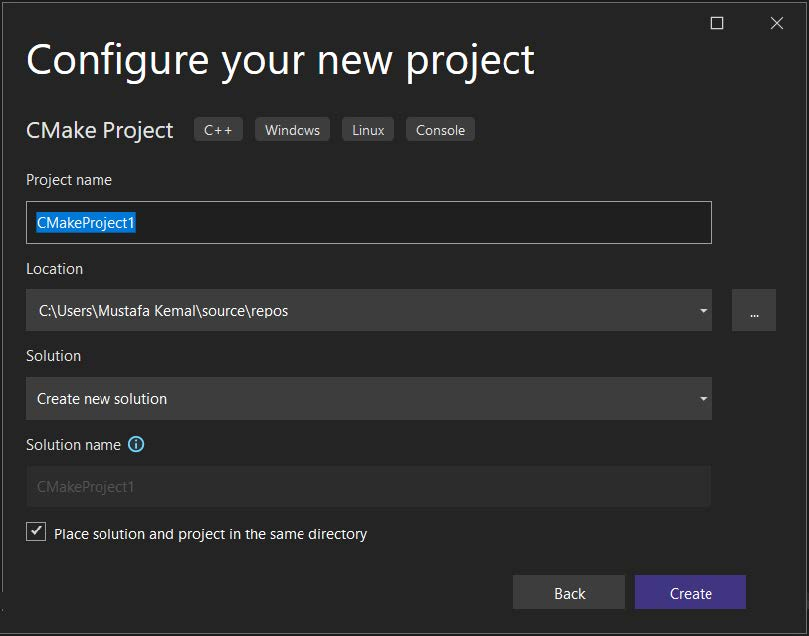
\includegraphics[width=0.8\textwidth]{content/1/chapter2/images/37.jpg}\\
图2.37  Visual Studio 2022新项目配置界面
\end{center}

填写详细信息后,单击Create创建新的CMake项目。生成的项目将包含一个顶级的CMakeLists.txt文件,一个C++源文件,和一个C++头文件,以所选的项目名称命名。新建的项目布局如下图所示:

\begin{center}
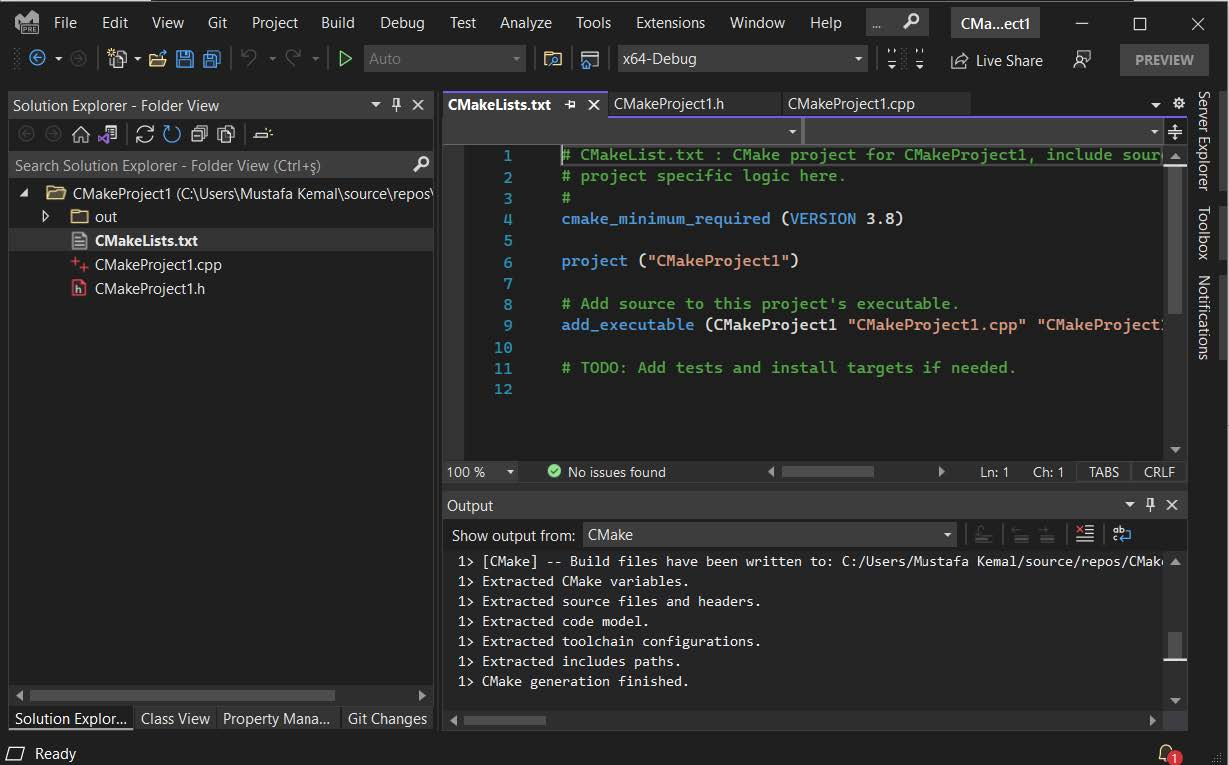
\includegraphics[width=0.8\textwidth]{content/1/chapter2/images/38.jpg}\\
图2.38 用Visual Studio创建的新的CMake项目
\end{center}

\hspace*{\fill} \\ %插入空行
\noindent
\textbf{打开已有的CMake项目}

打开现有的CMake项目,\texttt{File | Open | CMake...}并选择待打开项目的顶层CMakeLists.txt文件。下图显示了“打开”菜单的样子:

\begin{center}
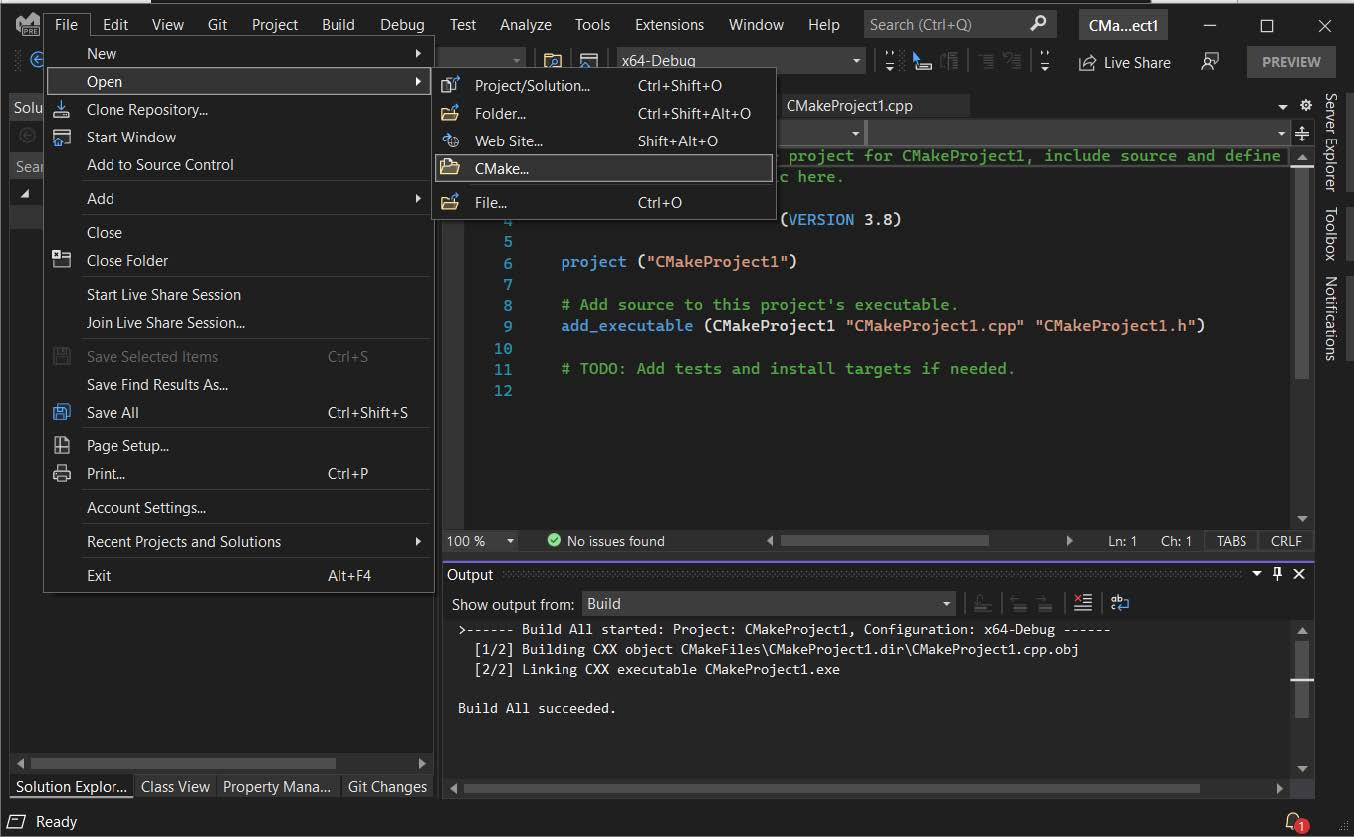
\includegraphics[width=0.8\textwidth]{content/1/chapter2/images/39.jpg}\\
图2.39 CMake项目打开菜单
\end{center}

接下来,让看看如何配置和构建CMake项目。

\hspace*{\fill} \\ %插入空行
\noindent
\textbf{配置和构建CMake项目}

要在Visual Studio中构建CMake项目,请先转到Project | Configure。这将调用CMake配置步骤并生成所需的构建系统文件。配置完成后,单击Build | Build All以生成项目。也可以通过使用F7快捷键来触发Build All。

注意,当保存CMakeLists.txt文件时,Visual Studio将自动重新配置,该文件是项目的一部分。

\hspace*{\fill} \\ %插入空行
\noindent
\textbf{使用CMake目标执行通用操作}

Visual Studio使用启动目标的概念来执行目标所需的操作,比如构建、调试和启动。要将CMake目标设置为启动目标,请使用工具栏上的“选择启动目标”下拉框。Visual Studio将自动在配置中使用CMake目标填充这个下拉框。

\begin{center}
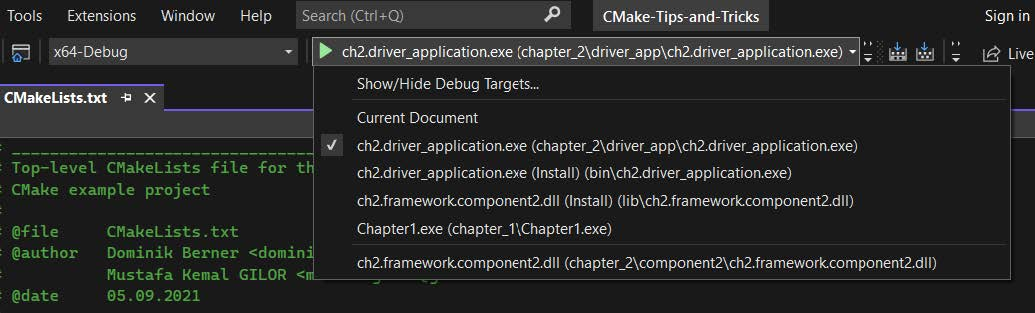
\includegraphics[width=0.8\textwidth]{content/1/chapter2/images/40.jpg}\\
图2.40 启动目标的下拉菜单
\end{center}

设置启动目标后,可以使用诸如调试、构建或启动等操作:

\begin{itemize}
\item 
要调试,首先单击“Debug | Startup Target”,然后单击“Debug | Start Debugging”或使用F5快捷键。

\item 
要在不调试的情况下启动,单击“ Start without debug”或使用Ctrl + F5快捷键。

\item 
要构建,单击Build,或单击Build | Build <target>,或使用Ctrl + B键盘快捷键。

\item
按钮位置如下图所示:

\begin{center}
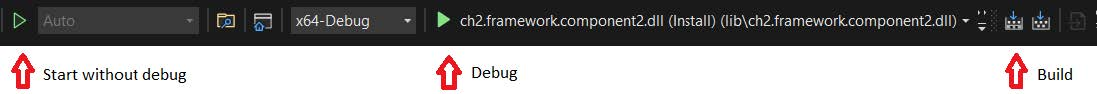
\includegraphics[width=0.8\textwidth]{content/1/chapter2/images/41.jpg}\\
图2.41 工具栏按钮的位置
\end{center}
\end{itemize}

本节中,已经介绍了Visual Studio CMake集成的基础知识。下一节中,将继续了解另一个微软产品,Visual Studio Code。

\subsubsubsection{2.4.2\hspace{0.2cm}Visual Studio Code}

Visual Studio Code (VSCode)是微软开发的一款开源代码编辑器。它不是一个IDE,但可以很强大,并通过扩展具有类似IDE的特性。扩展市场有各种各样的附加内容,从主题到语言服务器。可以找到几乎任何东西的扩展,这使VSCode既强大,喜欢广泛的观众,VSCode也有一个官方的CMake扩展。这个扩展最初是由Colby Pike开发的(也称为vector-of-bool),但现在由微软官方维护。

本节中,将学习如何安装扩展并使用它执行基本的CMake任务。

在继续之前,VSCode必须已经安装在您的环境中。若还没装,请访问\url{https://code.visualstudio.com/learn/get-started/basics}了解下载和安装的详细信息。

此外,我们将经常访问命令面板。强烈建议经常使用来熟悉它,而命令面板是什么?下面是截图:

\begin{center}
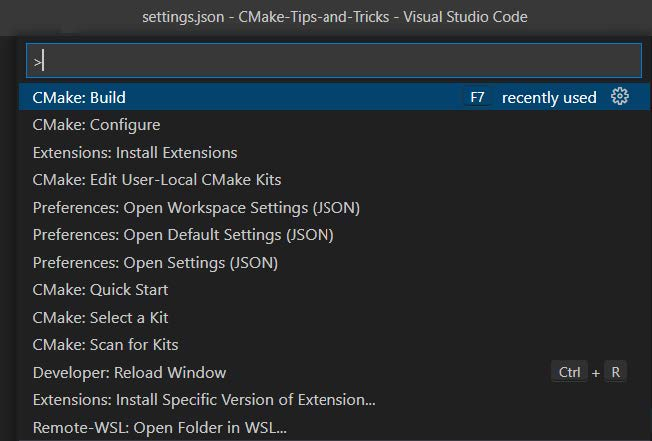
\includegraphics[width=0.6\textwidth]{content/1/chapter2/images/42.jpg}\\
图2.42 VSCode命令面板
\end{center}

说实话,我直到现在才知道它有名字。访问命令面板的快捷键是F1和Ctrl + Shift + p。命令面板是VSCode的面包和黄油,加快了VSCode的工作流程。

\hspace*{\fill} \\ %插入空行
\noindent
\textbf{安装扩展}

安装扩展是非常直接和简单的。要使用CLI安装它,调用以下命令(如果使用的是Insiders版本,则用code-insiders替换code):

\begin{tcblisting}{commandshell={}}
code --install-extension ms-vscode.cmake-tools
\end{tcblisting}

也可以在VSCode GUI中做同样的事情。打开VSCode,单击左侧导航窗格上的Extensions导航到Extensions页面。或者,您可以使用Ctrl + Shift + X快捷键。在扩展搜索框中键入CMake工具,从微软选择CMake工具。注意不要将它与CMake扩展混淆,然后按下安装按钮来安装。

\begin{center}
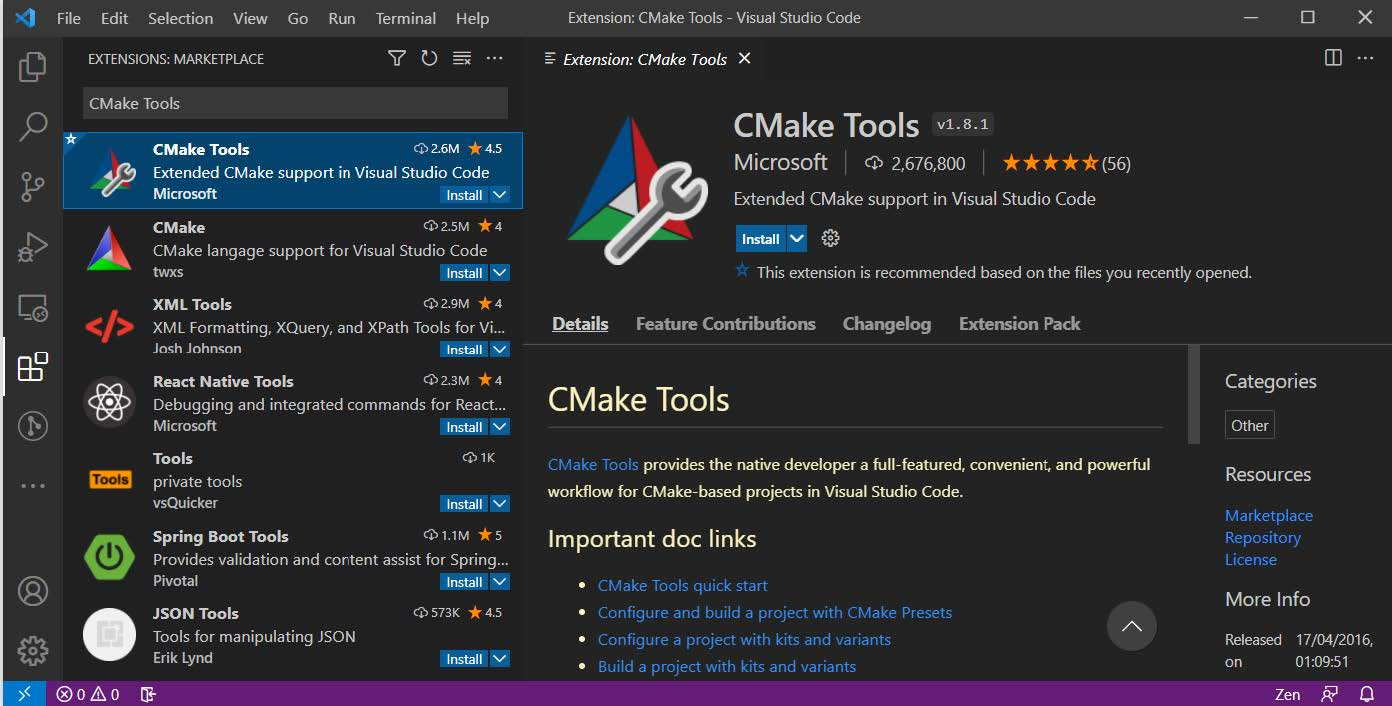
\includegraphics[width=0.8\textwidth]{content/1/chapter2/images/43.jpg}\\
图2.43  VSCode扩展市场
\end{center}

安装完成后,扩展就可以使用了。

\hspace*{\fill} \\ %插入空行
\noindent
\textbf{快速启动项目}

VSCode CMake工具扩展提供了一个快速启动选项,可以引导一个CMake项目,使用示例C++代码。要使用它,首先使用File | Open Folder…打开目标文件夹,然后按F1,并键入\texttt{cmake quick start}。选择“CMake: Quick Start”,按“Enter”键。

\begin{center}
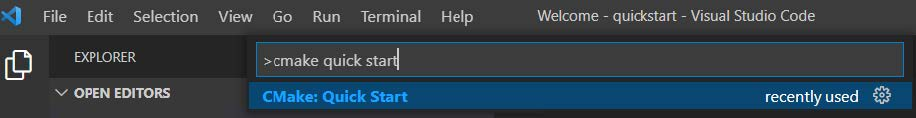
\includegraphics[width=0.8\textwidth]{content/1/chapter2/images/44.jpg}\\
图2.44 命令面板——定位CMake:快速入门
\end{center}

首先,扩展会询问使用哪个套件。选择适合新项目的选项。工具包将在处理工具包一节中会进一步讨论。

选择工具包之后,系统会要求输入项目名称,这将是顶层CMake项目的名称。

最后,将显示选择一个示例应用程序。选择中,将会要求创建一个可执行的应用程序项目或一个库项目。选择其中之一,然后创建CMake项目,CMakeLists.txt和main.cpp文件将自动生成。

\hspace*{\fill} \\ %插入空行
\noindent
\textbf{打开现有的项目}

VSCode中打开CMake项目没什么特别。打开包含项目顶层CMakeLists.txt文件的文件夹,CMake工具扩展将自动识别该文件夹为CMake项目,所有CMake相关的命令将在VSCode命令面板上可用。

\hspace*{\fill} \\ %插入空行
\noindent
\textbf{配置、构建和清理项目}

要配置CMake项目,从命令面板中选择CMake: Configure菜单项。要构建项目,通过从命令面板中选择CMake: Set build target菜单项来选择一个构建目标,可以选择在调用构建时构建的内容。最后,选择CMake: Build来构建选定的构建目标。要生成一个特定的目标而不将其设置为生成目标,请使用CMake: build target菜单项。

要清理构建工件,使用CMake:Clean命令面板项。这将运行CMake的clean目标并删除所有构建工件。

\hspace*{\fill} \\ %插入空行
\noindent
\textbf{调试目标}

要调试一个目标,从命令面板中选择CMake: Set debug target菜单项来选择一个调试目标。会看到列出的可调试目标。

\begin{center}
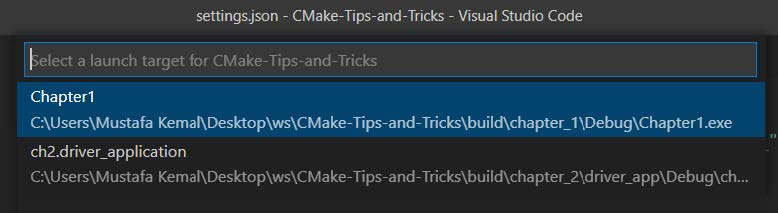
\includegraphics[width=0.8\textwidth]{content/1/chapter2/images/45.jpg}\\
图2.45 选择调试目标
\end{center}

选择目标并从命令面板中选择CMake: Debug (Ctrl + F5),所选目标将在调试器下启动。

若想在没有调试器的情况下运行选定的目标,选择CMake: run without Debugging (Shift + F5)。

\begin{center}
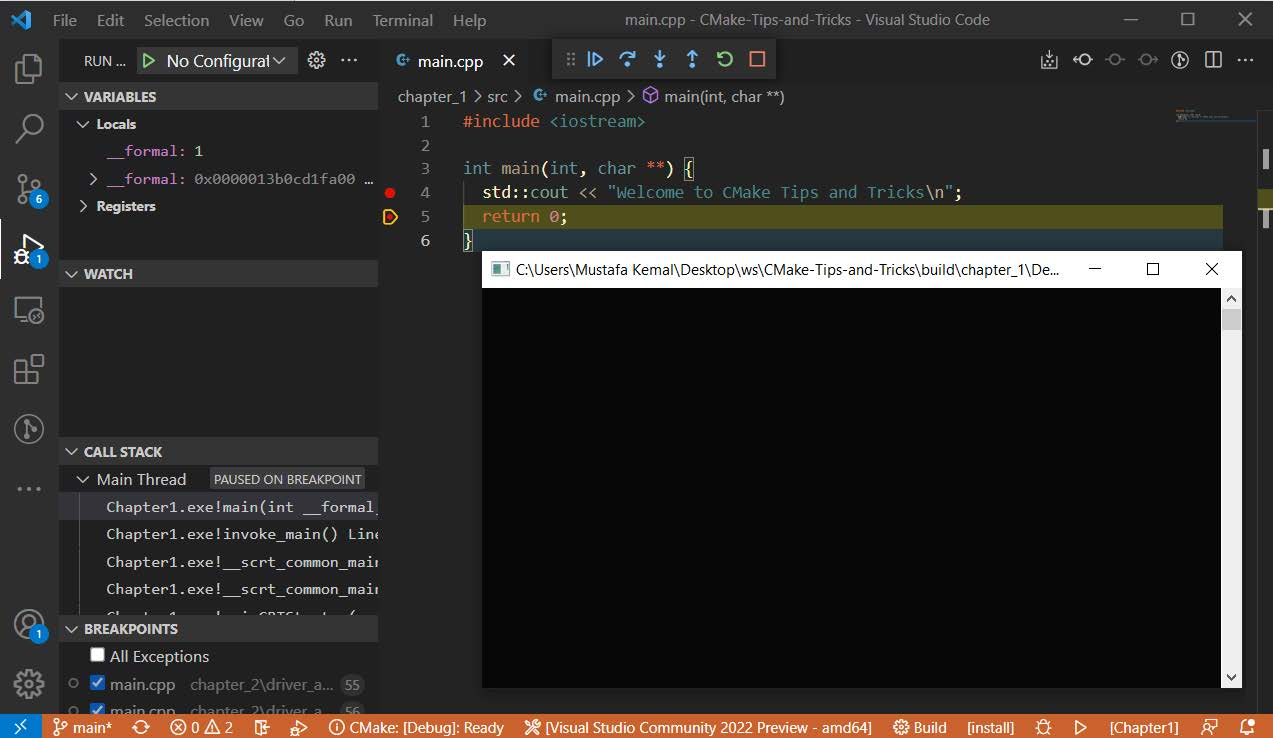
\includegraphics[width=0.8\textwidth]{content/1/chapter2/images/46.jpg}\\
图2.46 正在调试可执行的Chapter1目标
\end{center}

下一节中,将研究如何为已调试的目标提供参数。

\hspace*{\fill} \\ %插入空行
\noindent
\textbf{向调试的目标传递参数}

试图调试的目标可能需要命令行参数。要将命令行参数传递给调试目标,请打开VSCode的settings.json文件,并添加以下行:

\begin{lstlisting}[style=styleCMake]
"cmake.debugConfig": {
		"args": [
		"<argument1>",
		"<argument2>"
		]
	}
\end{lstlisting}

JSON中的args数组中,可以放置目标所需的任意数量的参数。这些参数将无条件地传递给所有未来的调试目标。若希望对参数进行更细粒度的控制,最好定义一个launch.json文件。

\hspace*{\fill} \\ %插入空行
\noindent
\textbf{处理套件}

A kit in the CMake Tools extension represents a combination of tools that can be used to build the project; hence, the term kit is pretty much a synonym for the toolchain. Kits make it easier to work in a multi-compiler environment, allowing a user to choose which exact compiler to work with. Kits can be discovered automatically by the extension, read from toolchain files, or defined by the user manually.

To see available kits for a project, select the CMake: Select a Kit menu item from the Command Palette (F1 or Ctrl+Shift+P).

\begin{center}
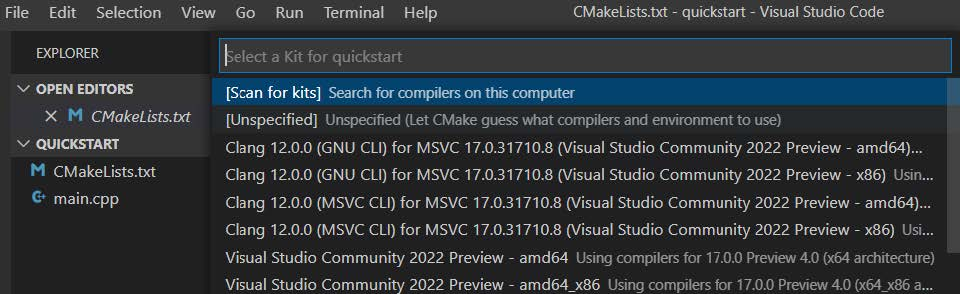
\includegraphics[width=0.8\textwidth]{content/1/chapter2/images/47.jpg}\\
图2.47 套件选择列表
\end{center}

The selected kit will be used for configuring the CMake project, which means the tools that are defined in the kit will be used for compiling the project. Kit selection will automatically trigger a CMake configuration.

By default, kits are scanned by the extension automatically. As a result, discovered toolchains are listed as options in the kit selection menu. If your toolchain is not displayed here, this means CMake Tools failed to discover it. In such a scenario, try to re-scan for kits first. If it is still missing, you can always define additional kits by adding them to the user-local cmake-tools-kits.json (1) file manually.

Adding a new kit is not usually necessary since the extension does a good job of discovering the toolchains. In the odd case of failure, there is a kit template here, which you can customize and append to the user-local cmake-tools-kits.json file to define a new kit. To open the user-local kits file, select the CMake: Edit User-Local CMake Kits menu item from the Command Palette:

\begin{lstlisting}[style=styleCMake]
{
	"name":"<name of the kit>",
	"compilers" {
		"CXX":"<absolute-path-to-c++-compiler>",
		"C": "<absolute-path-to-c-compiler>"
	}
}
\end{lstlisting}

\begin{tcolorbox}[colback=webgreen!5!white,colframe=webgreen!75!black,title=Note]
旧版本的CMake工具扩展,cmake-tools-kits.json文件可以命名为cmake-kits.json。
\end{tcolorbox}

Keep in mind that if your kit name collides with an autogenerated name from CMake Tools, CMake Tools will override your entry on a scan, so, always give unique names to your kit definitions.

For further information about kits, refer to \url{https://github.com/microsoft/vscode-cmake-tools/blob/develop/docs/kits.md}.

\subsubsubsection{2.4.3\hspace{0.2cm}Qt Creator}

Qt Creator is another IDE that supports CMake projects. CMake support is decent and the support comes out of the box without the need for any extra plugins. In this section, we are going to take a quick glance into Qt Creator's CMake support.

As always, ensure that you have the IDE installed and configured properly in your
environment first.

Qt Creator version 5.0.1 is used in the examples.

\hspace*{\fill} \\ %插入空行
\noindent
\textbf{Adding your CMake installation}

In order to use CMake with Qt Creator, the path of CMake must be defined in Qt Creator. To view and define CMake paths, navigate to Tools | Options | Kits | CMake.

\begin{center}
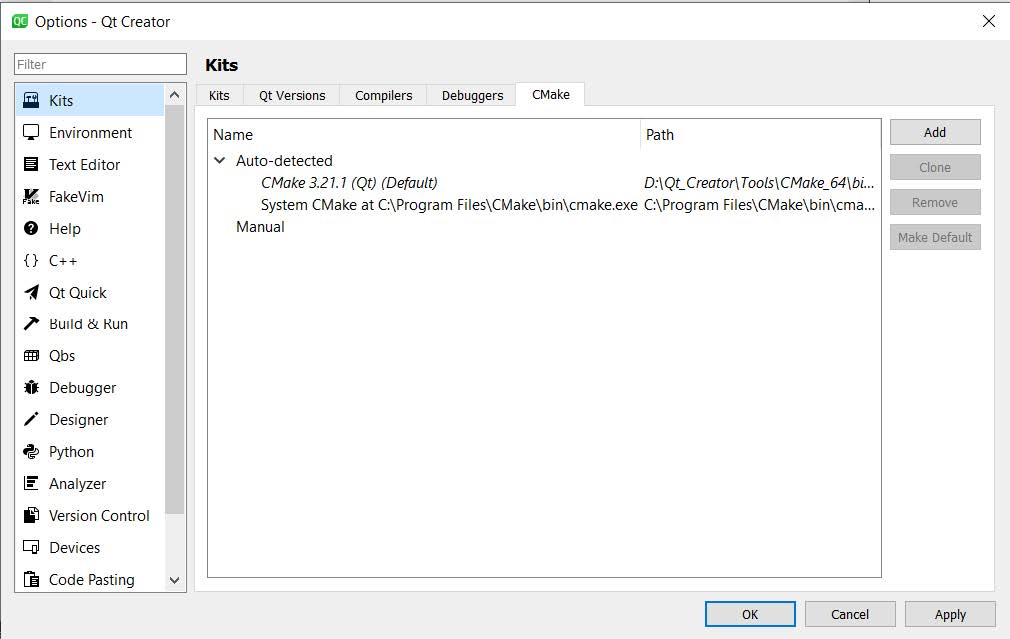
\includegraphics[width=0.8\textwidth]{content/1/chapter2/images/48.jpg}\\
Figure 2.48 – Qt Creator CMake path settings
\end{center}

Albeit with a lack of any manual definition, Qt Creator was able to discover CMake installations in the system. The first entry under the Auto-detected section is the CMake executable shipped together with Qt Creator. The second one is the system's CMake installation. To select which CMake executable to run in Qt Creator, select the desired entry and click the Make Default button.

To add a new CMake executable, click Add. This will append a new entry in the Manual section and bring up a window to fill in the details for the new entry.

\begin{center}
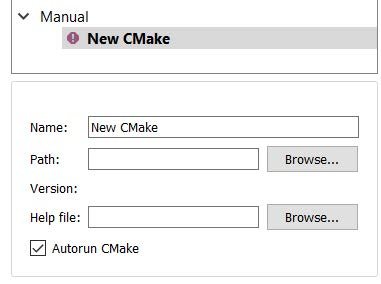
\includegraphics[width=0.6\textwidth]{content/1/chapter2/images/49.jpg}\\
Figure 2.49 – Adding a new CMake executable
\end{center}

The window fields are described in detail here:

\begin{itemize}
\item 
Name: A unique name to distinguish a new CMake executable entry.

\item 
Path: A CMake executable path (cmake/cmake.exe).

\item 
Version: The version of the CMake (deduced by Qt Creator).

\item 
Help file: An optional Qt Creator help file for the executable. This will allow CMake Help to appear upon pressing F1.

\item 
Autorun CMake: Check this to run CMake automatically on any CMakeLists.txt file changes.
\end{itemize}

After filling in the details, click Apply to add the new CMake executable to Qt Creator. Don't forget to set it as default if you intend Qt Creator to use it.

\hspace*{\fill} \\ %插入空行
\noindent
\textbf{Creating a CMake project}

Creating a CMake project in Qt Creator follows the exact same steps as for regular project creation. Qt Creator does not treat CMake as an external build system generator. Instead, it lets its users choose between three build system generators, which are qmake, cmake, and qbs. Any type of Qt project can be started by any of these build system generators from scratch.

To create a CMake project in Qt Creator, click File | New File or Project... (Ctrl + N) and choose the type of project from the New File or Project window. We'll go with Qt Widgets Application for our example.

\begin{center}
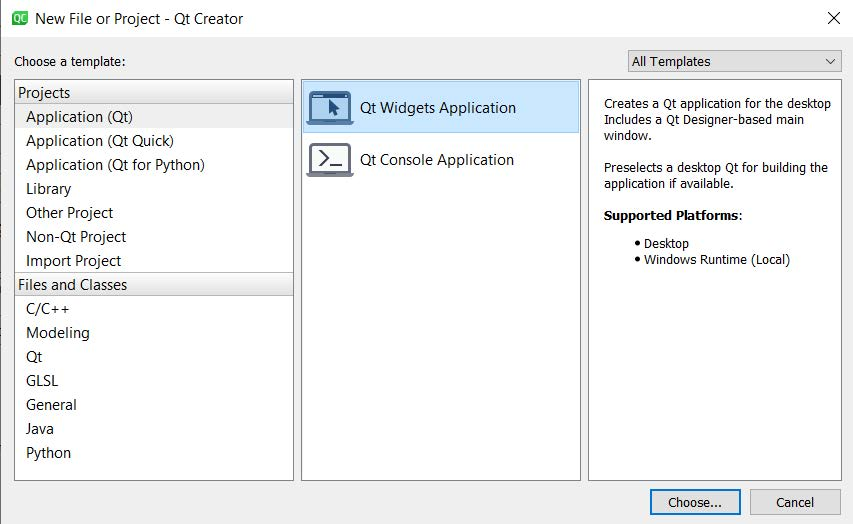
\includegraphics[width=0.8\textwidth]{content/1/chapter2/images/50.jpg}\\
Figure 2.50 – Qt Creator New File or Project window
\end{center}

Upon selection, the project creation wizard will appear. Fill in the details as desired. Select CMake in the Define Build System step, as shown in the following screenshot:

\begin{center}
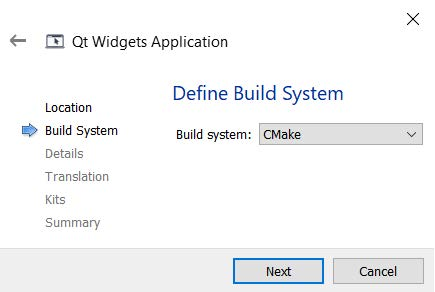
\includegraphics[width=0.6\textwidth]{content/1/chapter2/images/51.jpg}\\
Figure 2.51 – Qt Creator new project wizard build system selection
\end{center}

That's it! You've got yourself a Qt application with the CMake build system.

The following figure shows a newly created CMake project:

\begin{center}
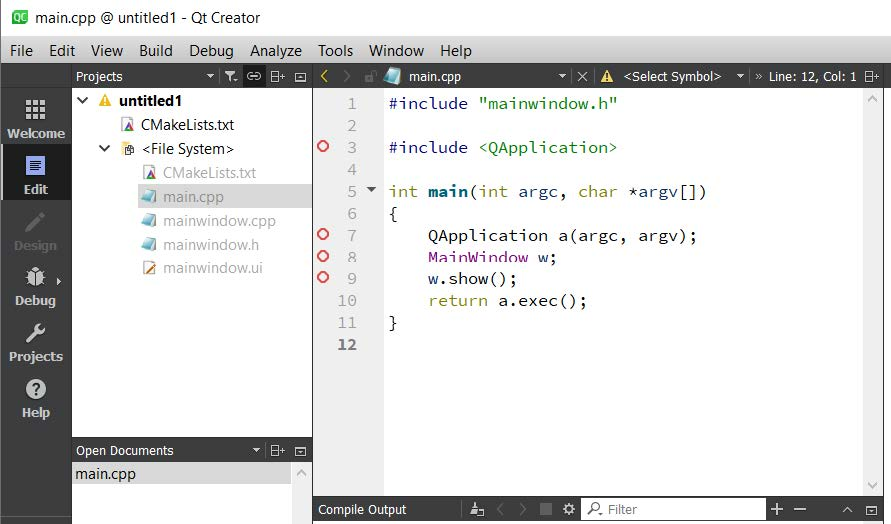
\includegraphics[width=0.8\textwidth]{content/1/chapter2/images/52.jpg}\\
Figure 2.52 – Generated CMake-based Qt widgets application project
\end{center}

\hspace*{\fill} \\ %插入空行
\noindent
\textbf{Opening an existing CMake project}

To open an existing CMake project with Qt Creator, go to the File | Open File or Project... (Ctrl + O) menu item. Select the top-level CMakeLists.txt file of the project and then click Open. Qt Creator will prompt you to choose a kit for your project. Select your preferred kits and then click on the Configure Project button. The project will be open and the CMake configure step will be run with the selected kits.

As an example, the CMake Best Practices project opened with Qt Creator is shown in this figure:

\begin{center}
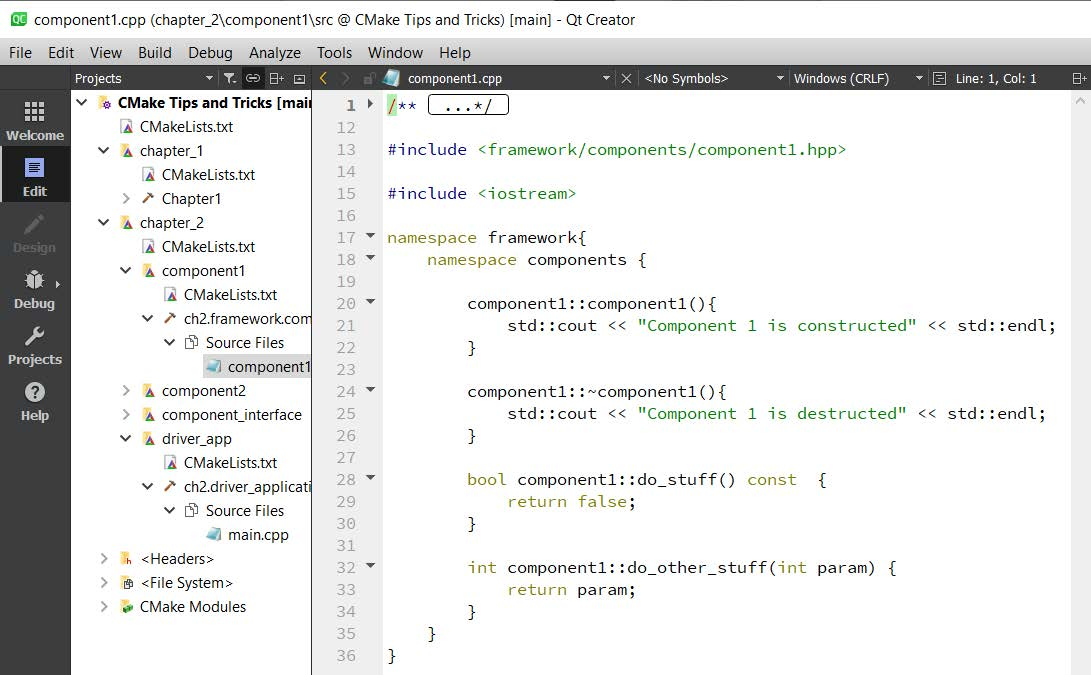
\includegraphics[width=0.8\textwidth]{content/1/chapter2/images/53.jpg}\\
Figure 2.53 – A glance at the CMake Tips and Tricks example project in Qt Creator
\end{center}

After opening a CMake project for the first time, Qt Creator will create a file named CMakeLists.txt.user in the project's root directory. This file contains Qt-specific details that cannot be stored in the CMakeLists.txt file, such as kit information and editor settings.

\hspace*{\fill} \\ %插入空行
\noindent
\textbf{Configuring and building}

In most scenarios (for example, project opening and saving changes to CMakeLists.txt), Qt Creator will run CMake configuration automatically without having to run it manually. To run CMake configuration manually, click on the Build | Run CMake menu item.

After configuration, press the hammer icon in the left-most corner to build the project. Alternatively, the Ctrl + B keyboard shortcut can be used. This will build the whole CMake project. To build a specific CMake target only, use the Locator next to the Build button. Type cm and then press the space bar on your keyboard.

\begin{center}
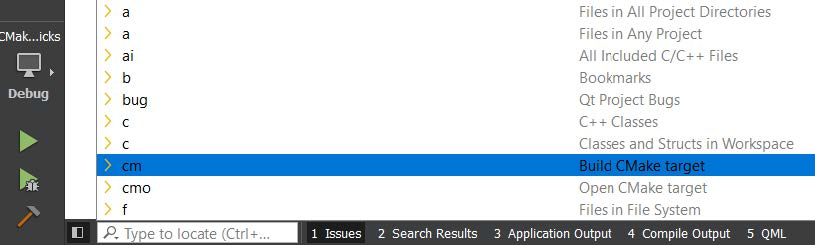
\includegraphics[width=0.8\textwidth]{content/1/chapter2/images/54.jpg}\\
Figure 2.54 – Qt Creator locator suggestions
\end{center}

The locator will display CMake targets available to build. Select the desired target either by highlighting it and pressing Enter, or by clicking on it directly using the mouse.

\begin{center}
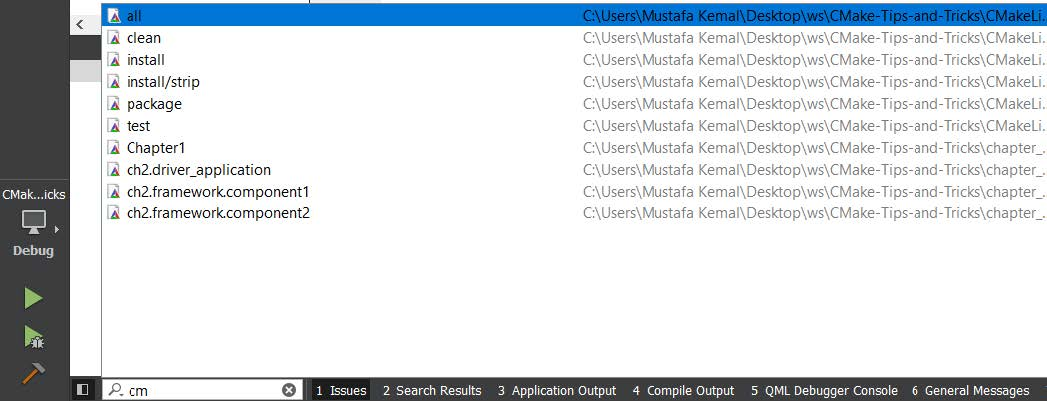
\includegraphics[width=0.8\textwidth]{content/1/chapter2/images/55.jpg}\\
Figure 2.55 – Available CMake targets to build displayed on the locator
\end{center}

The selected CMake target (and naturally, its dependencies) will be built.

\hspace*{\fill} \\ %插入空行
\noindent
\textbf{Run and debug}

To run or debug a CMake target, press the kit selector button (the computer icon on the left navigation bar) and select the CMake target. Then, click either the run button (the play icon under the kit selector) to run or the debug button (the play icon with a bug) to debug.

The following figure shows the kit selector menu content:

\begin{center}
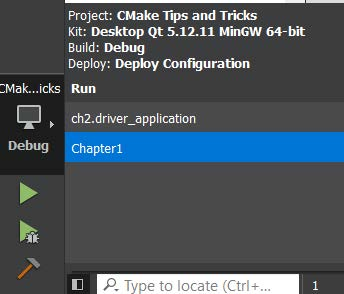
\includegraphics[width=0.5\textwidth]{content/1/chapter2/images/56.jpg}\\
Figure 2.56 – Kit selector displaying CMake targets
\end{center}

Here, we conclude the basics of using CMake with Qt Creator. For more advanced topics, you can consult the resources given in the Further reading section.

















